\documentclass[12pt]{article}

%AMS-TeX packages
\usepackage{amssymb,amsmath,amsthm} 
%geometry (sets margin) and other useful packages
\usepackage[margin=1.25in]{geometry}
\usepackage{graphicx,ctable,booktabs}


%Redefining sections as problems
%
\makeatletter
\newenvironment{problem}{\@startsection
       {section}
       {1}
       {-.2em}
       {-3.5ex plus -1ex minus -.2ex}
       {2.3ex plus .2ex}
       {\pagebreak[3]%forces pagebreak when space is small; use \eject for better results
       \large\bf\noindent{Problem }
       }
       }
       {%\vspace{1ex}\begin{center} \rule{0.3\linewidth}{.3pt}\end{center}}
       \begin{center}\large\bf \ldots\ldots\ldots\end{center}}
\makeatother


%
%Fancy-header package to modify header/page numbering 
%
\usepackage{fancyhdr}
\pagestyle{fancy}
%\addtolength{\headwidth}{\marginparsep} %these change header-rule width
%\addtolength{\headwidth}{\marginparwidth}
\lhead{Problem \thesection}
\chead{} 
\rhead{\thepage} 
\lfoot{\small\scshape CS124} 
\cfoot{} 
\rfoot{\footnotesize PA 1 Writeup} 
\renewcommand{\headrulewidth}{.3pt} 
\renewcommand{\footrulewidth}{.3pt}
\setlength\voffset{-0.25in}
\setlength\textheight{648pt}

%1%%%%%%%%%%%%%%%%%%%%%%%%%%%%%%%%%%%%%%%%%%%%%%

%
%Contents of problem set
%    
\begin{document}

\title{CS124: PA 1 Writeup}
\author{Wen-Yuan Yao & Aidan Daly}
\date{3/1/2012}
\maketitle
\thispagestyle{empty}

\begin{problem}{}
A table or graph listing the average tree size for serveral values of n.\\

\begin{tabular}{ | c | c | c |c|c|c|c|c|c|}
  \hline                        
  n & tree size (d=0) & tree size (d=2) & tree size (d=3) & tree size (d=4) \\
  \hline
  16&1.123377&2.614219&4.620937&6.154804\\
  32&1.190543&3.920853&7.014574&10.109425\\
  64&1.198439&5.439917&11.163415&16.806942\\
  128&1.202553&7.454933&17.744405&28.324339\\
  256&1.200512&10.591843&27.548595&47.191632\\
  512&1.212632&14.943216&43.167509&78.61608\\
  1024&1.207085&20.88873&67.914395&129.904617\\
  2048&1.201441&29.650405&106.8256&217.334303\\
  4096&1.204866&41.707788&169.495394&360.765859\\
  8192&1.204736&58.893669&267.092103&603.201892\\
  16384&1.203603&83.415146&422.686491&1010.222384\\
  32678&1.202094&117.378755&667.426134&1683.683395\\
  65356&1.202011&165.925924&1057.090013&2822.219143\\
  130712&&&1674.326863&4730.655547\\
  261424&&&&7937.682697\\
  \hline  
\end{tabular}\\

*All tree sizes were averaged over a minimum of 5 trials.

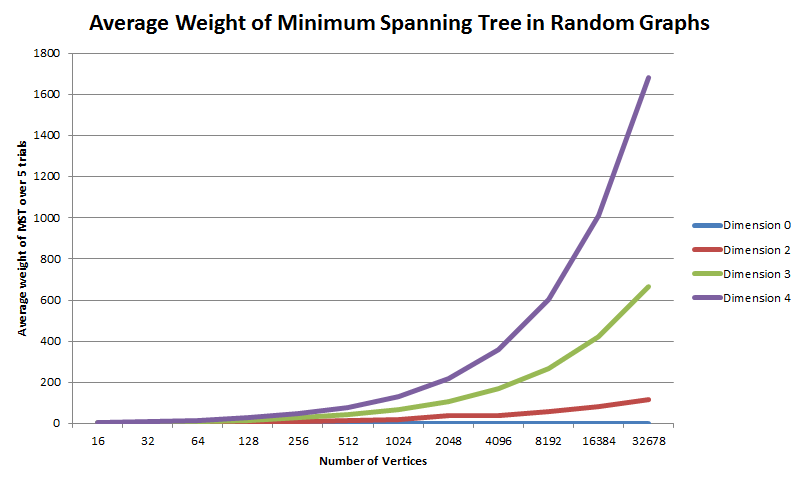
\includegraphics[height=90mm]{tree_size.png}

\end{problem}

\begin{problem}{}
A description of out guess for the function $f(n)$ and the reasoning
behind it.\\

\noindent The growth function for 0 dimensions (random weights)
quickly converges to roughly 1.2 for any significant number of vertices.\\

\noindent The growth function we determined for dimensions 1 or higher was:
\begin{equation}
f(n) = \frac{2}{3}\frac{n}{n^{1/k}}
\end{equation}
Where $k$ is the dimension of the problem.  The way we came to this function, which agrees very nicely with our empirical data, is as follows:\\

\noindent For any graph of size $n$, the minimum spanning tree will contain $n-1$ edges.  Thus, the total weight of the tree will obviously be proportional to $n$.  We figured that we could predict the weight of the tree by multiplying $n$ by the average weight of an edge we'd expect to be included in the tree.  We reasoned the average weight of such edges by first considering the one-dimensional case.\\

\noindent In the one-dimensional case, we'd expect nodes to be uniformly distributed on a line between 0 and 1.  Thus, we'd expect the average distance between any two adjacent nodes to be $\frac{1}{n}$.  Since the MST in 1 dimension is simply connecting all the adjacent nodes, we'd thus expect the average weight of an edge included in the MST to be $\frac{1}{n}$, which is consistent with our prediction.  Looking at the higher dimensional cases, it is still generally the case that edges added to the MST will be between "adjacent" nodes (i.e., edges between a node and its nearest neighbors).  We still expect points to be uniformly distributed in our unit shape at higher dimensions, and thus distance between a node and its nearest neighbors is still expected to be $\frac{1}{n^k}$.  Thus, assuming that edges are generally added between nodes and their nearest neighbors (which is generally true), the average weight of a node included in the MST will be $\frac{1}{n^k}$ in any dimension.\\

\noindent From our estimation, the growth function should be proportional to $\frac{n}{n^{1/k}}$, which indeed it is.  We found from empirical evidence that the constant scaling factor required to fit our data the best was $\frac{2}{3}$.\\

\noindent This is consistent with the expected size of the Euclidean
minimum spanning tree for large number of points determined by
J. Michael Steele:

$$c(d)*n^{\frac{d-1}{d}}\int{f(x)^{\frac{d-1}{d}}dx}$$
\begin{verbatim}
http://en.wikipedia.org/wiki/Euclidean_minimum_spanning_tree
\end{verbatim}
where $f(x)$ is the density of the probability function for picking
points, $d$ is the dimension, and $c(d)$ is a constant. In our case,
the probability distribution is uniform, so the integral term is
simply 1. Empirically, $c(d)=2/3$ for the values of $d$ that we look at.\\

\noindent As for the "0 dimensional case" (random weights), we would expect it to be roughly similar to the 1-dimensional case since all edges are chosen to have weights uniformly between 0 and 1.  Indeed, as our above formula predicted, the average weight of the MST in "0D" is constant with respect to $n$.  However, it seems to be bounded at 1.2 rather than $\frac{2}{3}$, which may be due to the fact that we are making a single draw from a uniform to determine the weight rather than taking the difference of two draws.

\end{problem}

\begin{problem}{}
Which algorithm did you use and why?\\

\noindent We chose to implement Kruskal's algorithm, which required us to implement a disjoint heap data structure and a sorting algorithm.  Our decision to use Kruskal's algorithm came out of a choice between the two most commonly used algorithms, which are both fairly feasible to implement - Kruskal's and Prim's.\\

\noindent Prim's algorithm has a better amortized runtime for dense
graphs, although the amortized runtime of its best reported
implementation ($O(E + VlogV)$) requires the programmer to implement a
Fibonacci heap, which is a rather daunting task.  Kruskal's algorithm
has the benefit of using simpler data structures, and in general
graphs its $O(ElogV)$ runtime is not too shabby. The sort we
implemented was an iterative merge sort, $O(nlog n)$, which operated
on an array of edges. Additionally, the 
disjoint set data structure and the sort that we had to implement
would be good targets for optimization, which will be discussed next. 

\end{problem}

\begin{problem}{}
Optimizations that we performed.\\

\noindent For the disjoint set, we implemented it as a tree (as
discussed in class) utilizing path compression for the traversal
operations to amortize future lookups. We also performed a series of
constant factor optimizations, such as using logical shifts for
multiplications and simplifying the n choose 2 formula. But the most
significant optimization came from the hint to throw out edges.\\

\noindent While we knew we would be testing complete graphs, we also knew that due to the uniform random distribution of the points/weights, we would be able to throw out a significant number of edges before running Kruskal's algorithm.  Within the same dimension, as the number of vertices increased, we noticed the maximum weight of an edge included in the spanning tree decreased in a predictable fashion.  This was because as more nodes are added to a complete graph with uniformly random weights (or weights derived from uniformly random points), there is a higher chance of finding a shorter path that spans a given node.  By running multiple iterations of our algorithm on graphs of varying size and dimension, we were able to fit a size-dependent threshold function for each dimension that would give a ceiling for the weights of edges that could be included in the minimum spanning tree (shown below).\\

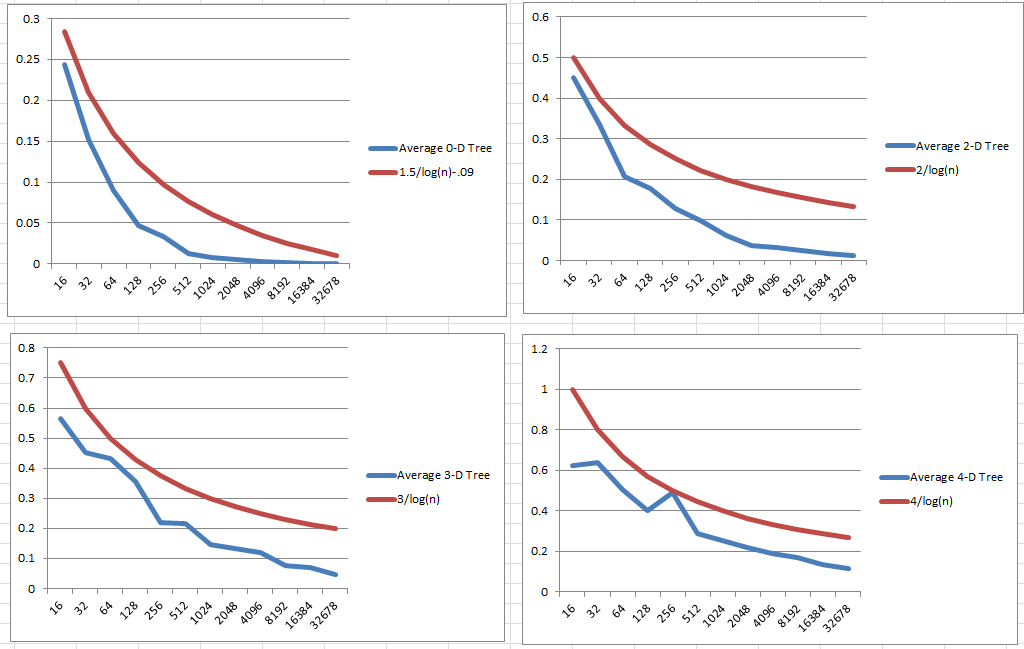
\includegraphics[height=90mm]{threshold.png}

\noindent As it turned out, the maximum weight of any edge added to a
minimum spanning tree was well bounded by a function proportional to
$\frac{d}{log(n)}$, where $n$ is the number of nodes in the function
and $d$ was the dimension of the graph. We used
$k(n)=\frac{d}{log(n)}$ directly for dimension 2-4 as a threshold
beyond which edges were discarded. For dimension 0, we used a modified
$k(n) = 1.5/log(n)-.09$ for $n \leq 32678$ in order to get a tighter
bound, and revert to the more conservative $k(n)=\frac{1}{log(n)}$ for
larger values of $n$.\\

\noindent Thus, as our program generates graphs, it automatically
discards edges with weights above the value of the threshold function.
This significantly reduced the size of the problem, improving both the
space and runtime efficiency of Kruskal's algorithm while maintaining
correctness with high probability. Note that the data for $n=256$ in
dimension 4 witnessed a maximum edge weight that approached (but did
not exceed) our threshold formula, showing that outliers are in fact possible, but
highly unlikely.

\end{problem}

\begin{problem}{}
How long does it take Kruskal's to run? Does this make sense??\\

\begin{tabular}{ | c|c|c|c | c | c |c|}
  \hline                        
  n & sec (d=0) & edge & c*E*log(V) & sec (d=2) & edge & c*E*log(V) \\
  \hline
16&0.0000062&39&4.0945E-06&0.0000088&56&5.87928E-06\\
32&0.0000168&107&1.4042E-05&0.0000232&173&2.27035E-05\\
64&0.0000472&323&5.08663E-05&0.0000764&514&8.09451E-05\\
128&0.0001306&1016&0.000186667&0.0002242&1619&0.000297455\\
256&0.000453&3223&0.000676747&0.0007438&5014&0.001052812\\
512&0.0015844&10055&0.002375204&0.0028298&16530&0.003904736\\
1024&0.0053194&31595&0.008292676&0.010198&55576&0.014586922\\
2048&0.0190424&96999&0.028005047&0.172993&615562&0.17772186\\
4096&0.0745774&293764&0.092524379&0.1753068&629938&0.19840628\\
8192&0.2326272&851237&0.290449215&0.6975154&2182371&0.744643317\\
16384&0.6888054&2301431&0.845672788&2.5632244&7596986&2.79155201\\
32678&2.1071128&5353458&2.107109583&10.0606146&26549410&10.44979081\\
\hline  
\end{tabular}

c = 0.0000000262468
\vspace{8mm}

\begin{tabular}{ | c|c|c|c | c | c |c|}
  \hline                        
  n & sec (d=3) & edge & c*E*log(V) & sec (d=4) & edge & c*E*log(V) \\
  \hline
16&0.0000106&77&8.08401E-06&0.0000114&100&1.04987E-05\\
32&0.0000288&207&2.71654E-05&0.000028&260&3.41208E-05\\
64&0.0000718&563&8.86617E-05&0.0000794&647&0.00010189\\
128&0.0002206&1552&0.000285145&0.0002338&1749&0.00032134\\
256&0.0006594&4475&0.000939635&0.000678&4759&0.000999268\\
512&0.002264&13647&0.003223711&0.0021502&12815&0.003027175\\
1024&0.0074842&41047&0.010773524&0.0065112&36146&0.009487168\\
2048&0.0263436&129867&0.037494525&0.0216552&106117&0.030637548\\
4096&0.1074164&405929&0.127852047&0.0807276&312938&0.098563453\\
8192&0.4064378&1309708&0.446883371&0.2599016&945328&0.322553854\\
16384&1.5266134&4302869&1.581111589&0.8938462&2912150&1.070084661\\
32678&5.3114222&14170888&5.577631113&3.000166&9082067&3.574682085\\
  \hline  
\end{tabular}

c=0.0000000262468
\vspace{5mm}

\noindent The times recorded here are only for Kruskal's algorithm and do not
include the time it takes to randomly generate edge weights. We also
calculated the average overall time for an entire iteration of the
program (see how we output our data in last section), but we did not
include that data in this report. Note that the average number of
relevant edges that were not thrown out are also recorded.\\

\noindent Our recorded runtimes correspond precisely to the theoretical runtime
of $O(E log(V))$. Using a scaling factor of $0.0000000262468$, our
runtimes very closely match theory, particularly for large values of $n$.

\end{problem}

\begin{problem}{}
Did you have any interesting experiences with the random number
generator? Do you trust it?\\

\noindent When we first wrote our code, we seeded the random number generator with the C system time.  This worked fine for single runs on a graph of a given size (or multiple runs on graphs of large size), but ended up producing the same ``\random" values for repeated iterations of small graph sizes.  This was because the C system time is reported in seconds, and once we realized this we switched over to the posix ``gettimeofday()" function, which allowed us to seed our random number generator with system time in microseconds times system time in seconds.  While this works for our purposes (we empirically tested on small cases to make sure this was generating a good degree of randomness), it is less than ideal to have a ceiling on how fast our program can run and still produce "random" output.  

\end{problem}

\begin{problem}{}
Final points of interest.\\

\noindent For dimension 4, we were able to get results up to 261,424 vertices in
545 seconds from edge generation to Kruskal's. Other results beyond 32,678
vertices are listed in the very first table. We were able to solve for
larger number of vertices in higher dimensions because they enjoyed
the function $k(n)$ used to throw out edges enjoyed a tighter bound. Presumably if
we taylored $k(n)$ for dimensions 0 and 2, they too could have been
solved at higher number of vertices.\\

\noindent Per problem set spec, the usage is:
\begin{verbatim}
randmst <opcode> <numpoints> <numtrials> <dimension>
\end{verbatim}
\noindent An opcode of 0 runs regularly to test for the average tree
sizes. The output is in the form:
\begin{verbatim}
<dimension>,<vertices>,<average tree size>,<average overall time>
\end{verbatim}
which can be piped directly into a csv file.\\
\noindent An opcode of 1  tests for the maximum edge weight. The output is in the form:
\begin{verbatim}
<dimension>,<vertices> ,<maximum edge weight>,<average overall time>
\end{verbatim}
\noindent An opcode of 2  tests for the average Kruskals run time
(omits generation) and the number of relevant edges. The output is in the form:
\begin{verbatim}
<edges>,<dimension>,<vertices>,<ave Kruskal's time>,<ave overall time>
\end{verbatim}

\end{problem}
%%%%%%%%%%%%%%%%%%%%%%%%%%%%%%%%%%%%%%%%%%%%%%%

\end{document}